\section{Runtime Inefficiencies}
\label{removal}

The identification and removal of inefficiencies follows the same iterative approach presented in section \ref{identification}.

\subsection{Multithreading Inefficiencies}

Without the sensibility provided by the tests in section \ref{identification}, a scientist would incur in the pitfall of using all available cores (and even all hardware threads) on the system, hoping that it would provide the best performance. While it may be true for the non-pointer implementation,the system computational resources would be used inefficiently, and using the single device highly efficient pointer implementation would induce a even greater waste.

Using multiple processes of the pointer implementation may provide better efficiency for NUMA systems. As it was not possible to refactor LipMiniAnalysis, which would be necessary to change the event information from a global to a private state and allow parallelizing the processing of multiple events, an MPI implementation.

Analysis applications are executed individually for each file (around 1GB in size) in a huge set of files, usually reaching the terabyte scale, received from CERN each week. An alternative approach to the MPI parallelization is to balance the execution of different \tth processes in the system on a set of input files. This reduces the complexity of the implementation, with no changes needed for \tth, and avoids communication between processes. A simple scheduler was devised, which takes a set of input files and creates a given amount of \tth processes. It is then responsible for dispatching the files to the different processes in a queue-like approach, and monitor their execution, as shown in figure \ref{fig:sched_flow}. A set of 20 input files was considered for testing purposes, with different configurations of processes and threads per process.

\begin{figure}[!htp]
	\begin{center}
		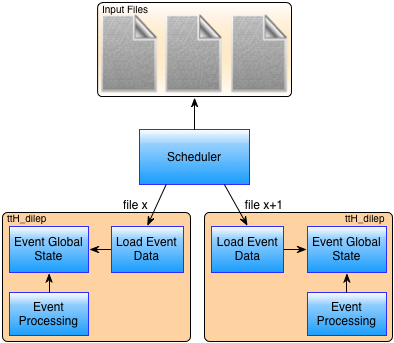
\includegraphics[scale=0.4]{images/scheduler_workflow.png}
		\caption{Schematic representation of dispatcher workflow.}
		\label{fig:sched_flow}
	\end{center}
\end{figure}

\begin{figure}[!htp]
	\begin{center}
		\raisebox{-0.5\height}{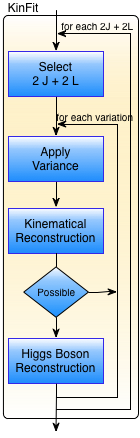
\includegraphics[scale=0.6]{images/sequential_kinfit.png}}
		\raisebox{-0.5\height}{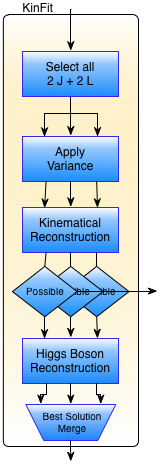
\includegraphics[scale=0.6]{images/parallel_kinfit.png}}
		\caption{Filler.}
		\label{fig:Sched}
	\end{center}
\end{figure}

Figure \ref{fig:Sched} presents the speedups using 2, 4, 5, 8, and 10 processes for different thread configurations to fill one or both CPU devices.

\subsection{Core Affinity Inefficiencies}

The final possible optimization at runtime regards the thread affinity, i.e., to which CPU cores a given thread is allocated. By default OpenMP allows for the Operating System to manage thread affinity, allowing for threads to be changed between cores during runtime. If a thread is running on core $c_1$ and it is moved to core $c_2$, all the data on the private cache $l_{c_1}$ needs to be reloaded to cache $l_{c_2}$, causing unnecessary overhead. This effect is amplified if the threads are moved between CPU devices. When multiple different, and possibly parallelized, processes are running on the same system, which is common in production environments, occurrences of bad scheduling occur more often.

Defining the thread affinity of an application may provide a more constant, or in some cases better, performance. In theory, an optimum thread affinity scheme allocates the threads to contiguous physical cores of one CPU device, uses the cores of the second CPU device only after the first is filled, and finally uses the multithreading after filling all physical cores. Note that using multithreading before the second CPU device may provide better performance in memory bound applications. This type of affinity must be defined prior to the application execution and depends on the system used. In this case the affinity was specifically tuned to this system for all threads, or process/threads configuration for the scheduler.

\begin{figure}[!htp]
	\begin{center}
		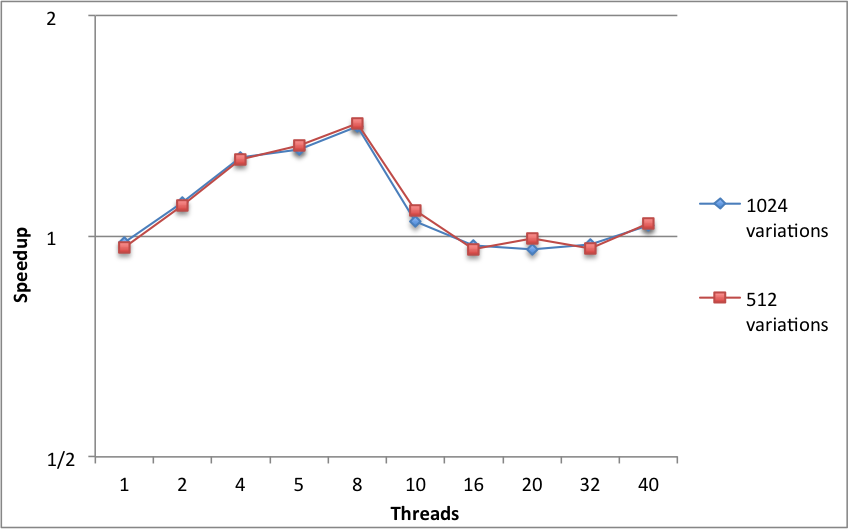
\includegraphics[scale=0.4]{charts/speedup_pointer_aff.png}
		\caption{Speedup of the \tth parallel pointer implementation with affinity \textit{vs} no affinity.}
		\label{fig:pointer_aff}
	\end{center}
\end{figure}

By analysing the speedups of the pointer implementation of \tth with thread affinity, in figure \ref{fig:pointer_aff}, it is concluded that specifying the affinity is best for a small number of threads, with speedups up to 1.2. It is a small improvement but provides a more constant and predictable application execution time. From an empirical analysis of the CPU devices at application runtime, the Operating System tends to move the threads more often when there are many unused cores. For a high number of threads, defining the affinity worsens the performance, with a insignificant speedup of 0.9.
